\documentclass{article}
\usepackage{fasy-hw}

\author{Joshua Harthan}
\problem{1}
\collab{Michael Valentino-Manno, Derek Jacobson}
\begin{document}
9.1 Question 22
\item[]a. How many positive three-digit integers are multiples of 6?
\item[]b. What is the probability that a randomly chosen positive three-digit integer is a multiple of 6?
\item[]c. What is the probability that a randomly chosen positive three-digit integer is a multiple of 7?


\problem{2}
\collab{none}
\clearpage
\header
9.2 Question 17
\item[]a. How many integers are there from 1000 through 9999?
\item[]b. How many odd integers are there from 1000 through 9999?
\item[]c. How many integers from 1000 through 9999 have distinct digits?
\item[]d. How many odd integers from 1000 through 9999 have distinct digits?
\item[]e. What is the probability that a randomly chosen four-digit integer has distinct digits? 


\problem{3}
\collab{none}\documentclass{article}
\usepackage{fasy-hw}

\author{Michael Valentino-Manno}
\problem{1}
\collab{Joshua Harthan, Derek Jacobson, Michael Valentino-Manno, Cayden Seiler, Joshua Freund}
\begin{document}
9.1 Question 22
\item[]\textbf{a.} "How many positive three-digit integers are multiples of 6?"
\item The set of three-digit integers are the integers from 100 to 999. The first one in that set that is a multiple of 6 is $102 = 6(17)$. The last one that's a multiple of 6 is $996 = 6(166)$. The difference between 166 and 17 is $166 - 17 - 149$, but since this doesn't count one of them (The number of elements in a list is equal to n - m + 1, with n and m being integers. e.g. $10 - 1 = 9$, but when including 1 and 10, there's not 9, but 10 numbers between 1 and 10), you must add one. $149 + 1 = 150$. So there's 150 positive three-digit integers that are multiples of 6.
\item[]\textbf{b.} "What is the probability that a randomly chosen positive three-digit integer is a multiple of 6?"
\item The total number of three-digit numbers is  $999 - 100 + 1 = 900$ numbers. Again, the "+ 1" is needed for the same reason as stated in part a. From part a, the number of three-digit numbers that are multiples of 6 is 150. Therefore the probability of a randomly chosen positive three-digit integer being a multiple of 6 is $\frac{150}{900} = \frac{30}{180} = \frac{1}{6}$.
\item[]\textbf{c.} "What is the probability that a randomly chosen positive three-digit integer is a multiple of 7?"
\item The amount of three-digit numbers that are multiples of 7 will be found the same way that it was found in part a. The smallest three-digit number that's a multiple of 7 is $15(7) = 105$. The largest three-digit number that's a multiple of 7 is $142(7) = 994$. So, the total number of three-digit numbers that are multiples of 7 is $142 - 15 + 1 = 128$. Again, the "+ 1" is needed for the same reason as stated in part a. From part b, the total number of three-digit numbers is 900. Therefore, the probability of a randomly chosen positive three-digit integer being a multiple of 7 is $\frac{128}{900} = \frac{64}{450} = \frac{32}{225}$.



\problem{2}
\collab{Joshua Harthan, Derek Jacobson, Michael Valentino-Manno, Cayden Seiler, Joshua Freund}
\clearpage
\header
9.2 Question 17
\item[]\textbf{a.} "How many ints are there from 1000 to 9999?"
\item From theorem 9.1.1 in the book, if a and b are integers and $a \leq b$, the number of integers in a list is equal to $b - a + 1$. So, the number of integers from 1000 to 9999 is $9999 - 1000 + 1 = 9000$.

\item[]\textbf{b.} "How many odd ints are there from 1000 to 9999?:
\item Since even and odd numbers alternate and our list starts at an even number, and ends at an odd number, the number of even numbers equals the number of odd numbers (e.g. from 2 to 3 there's an equal number of even and odds, but from 2 to 4, there's 2 even number and 1 odd number). So there are $\frac{9000}{2} = 4500$ odd numbers from 1000 to 9999.

\item[]\textbf{c.} "How many ints from 1000 to 9999 have distinct digits?"
\item In the range from 1000 to 9999, there can't be a 0 in the first position. So there's 9 digits that could be in the first position. Since the digit in the second position can include 0, but can't include what was in the first position, there's 9 digits it can be. Since the digit in the third position can't be either of the first two digits, and there's originally 10 possible digits, there is 10-2 possibilities for digits that can be in the third position. Finally, since the final digit can't be any of the previous 3, there's 10 - 7 possibilities for it. Therefore, the number of integers from 1000 to 9999 that have distinct integers is $9(9)(8)(7) = 4536$.

\item[]\textbf{d.} "How many odd ints from 1000 to 9999 have distinct digits?"
\item There are only 5 odd digits, and therefore the last position has 5 possibilities. With this requirement, there's only 8 possibilities for the first digit, since 0 and the already chosen odd digit can't occur again. The second can be 0, but not one of the other two digits. Therefore there's 8 possibilities for it. As for the third digit, it can't be any of the other 3. So there's 7 possibilities for it. Therefore there's $5(8)(8)(7) = 2240$ integers from 1000 to 9999 that is odd with distinct integers.

\item[]\textbf{e.} "What is the probability that a randomly chosen four-digit integer has distinct digits? Distinct digits and odd?"

\item From part a, there's 9000 four digit numbers, and from parts c and d, there's 4536 four-digit numbers with distinct digits, and 2240 odd four-digit numbers with distinct digits. So using these numbers, the probability that a randomly chosen number has distinct digits and  is four-digits long $\frac{4536}{9000} = \frac{63}{125}$. The probability that a randomly chosen, odd, four-digit number with distinct digits is chosen is $\frac{2240}{9000} = \frac{56}{225}$.


\problem{3}
\collab{Joshua Harthan, Derek Jacobson, Michael Valentino-Manno, Cayden Seiler, Joshua Freund}
\clearpage
\header
9.3 Question 32
\item[]"A study was done to determine the efficacy of three different drugs -$A, B,$ and $C$- in relieving headache pain. Over the period covered by the study, 50 subjects were given the chance to use all thee drugs. The following results were obtained":
\item[]"21 reported relief from drug $A$."
\item[]"21 reported relief from drug $B$."
\item[]"31 reported relief from drug $C$."
\item[]"9 reported relief from both drugs $A$ and $B$."
\item[]"14 reported relief from both drugs $A$ and $C$."
\item[]"15 reported relief from both drugs $B$ and $C$."
\item[]"41 reported relief from at least one of the drugs.
\item[]Note that some of the 21 subjects who reported relief from drug $A$ may also have reported relief from drugs $B$ or $C$. A similar occurrence may be true for the other data."
\item[]a. "How many people got relief from none of the drugs?"

From the difference rule, the number of people who got relief from none of the drugs is the difference of the number of total people in the study and the number of people who reported relief in at least one of the drugs; therefore, the number of people who got relief from none of the drugs is 50 - 41 = 9.

\item[]b. "How many people got relief from all three drugs?"

Let $A$ be the set of all subjects who got relief from drug $A$, $B$ the set of all subjects  who got relief from drug $B$, and $C$ the set of all subjects  who got relief from drug $C$. By the inclusion/exclusion rule, $N(A \cup B \cup C) = N(A) + N(B) + N(C) - N(A \cap B) - N(A \cap C) - N(B \cap C) + N(A \cap B \cap C)$ . Putting in values, we get 41 = 21 + 21 + 31 - 9 - 14 - 15  $+ N(A \cap B \cap C)$. Solving for $+ N(A \cap B \cap C)$, we get a value of 6. Therefore, the amount of people who got relief from all three drugs is six people. 

\problem{3 parts c and d}
\collab{Joshua Harthan, Derek Jacobson, Michael Valentino-Manno, Cayden Seiler, Joshua Freund}
\clearpage
\header
\item[]c. "Let $A$ be the set of all subjects who got relief from drug $A$, $B$ the set of all subjects  who got relief from drug $B$, and $C$ the set of all subjects  who got relief from drug $C$. Fill in the numbers for all eight regions of the diagram below":

\begin{figure}[h!]
  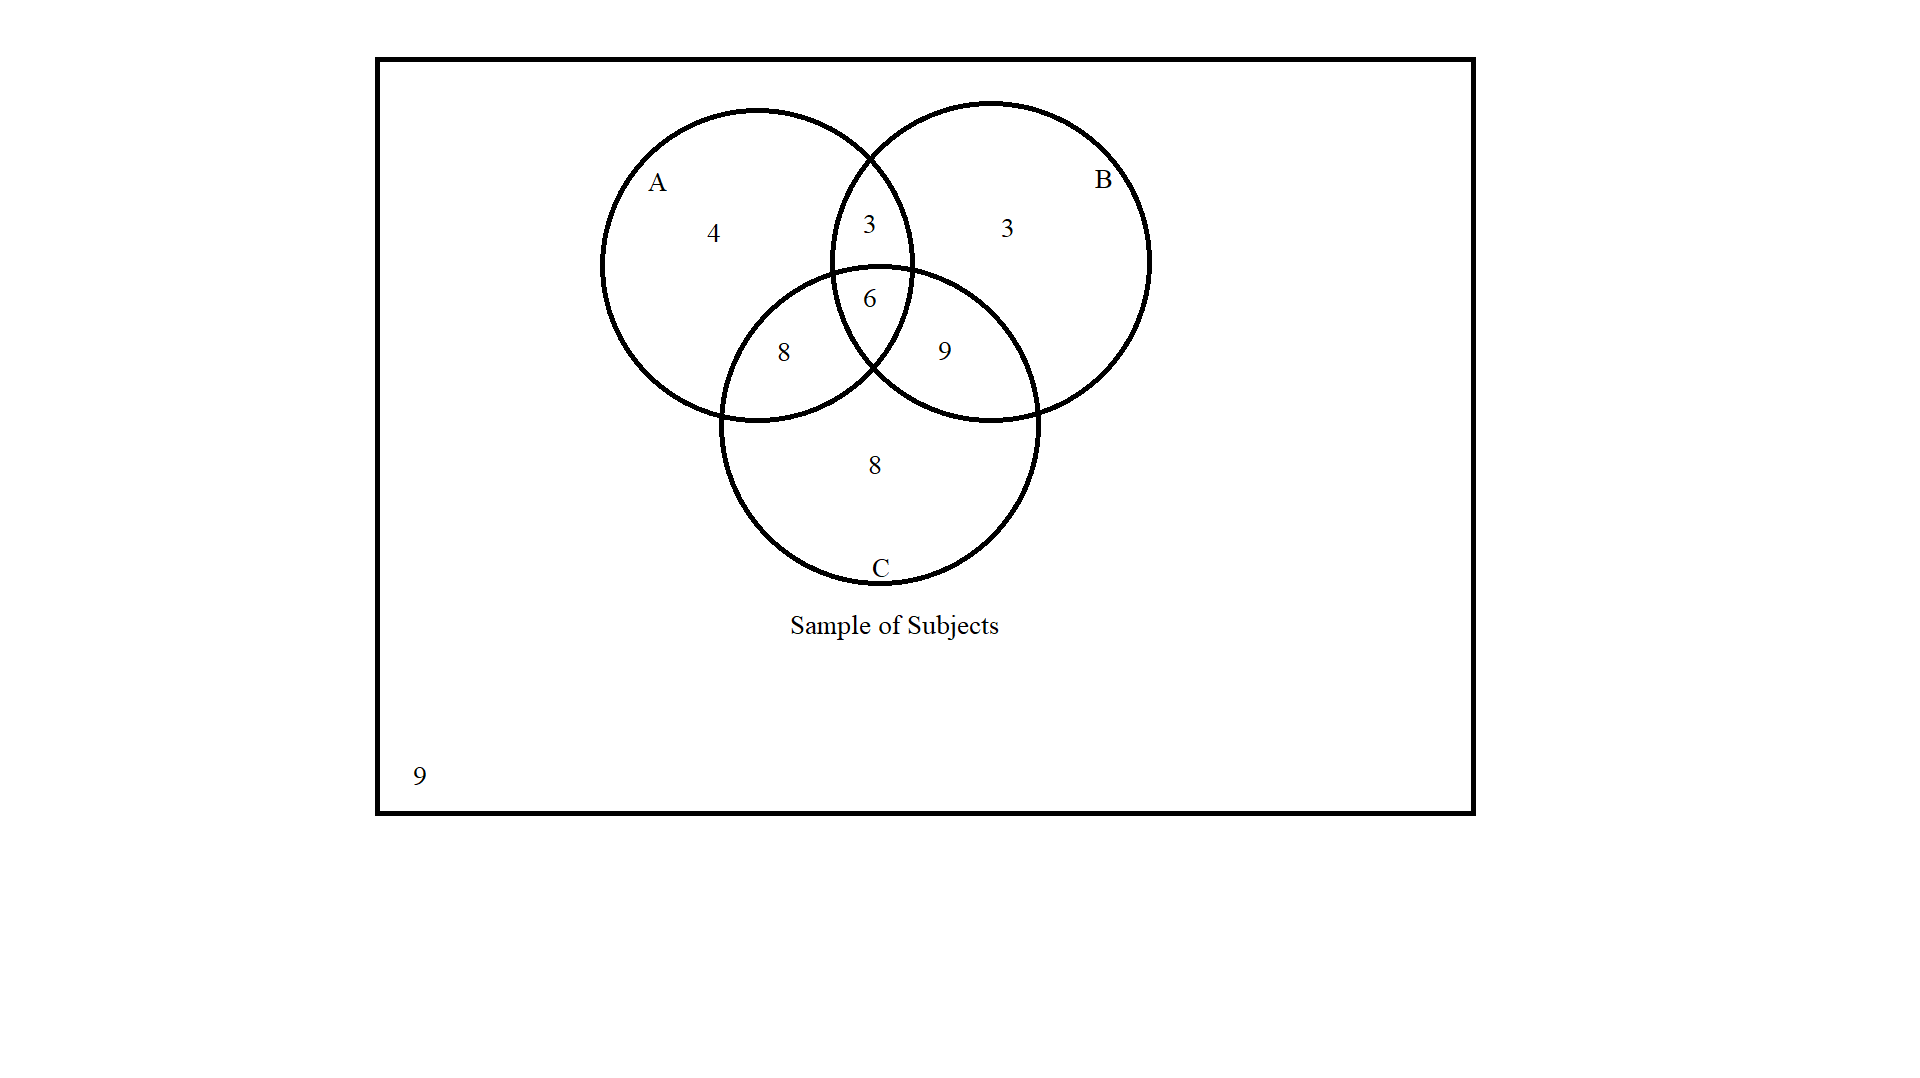
\includegraphics[width=\linewidth]{Untitled.png}
  \caption{Venn Diagram}
  \label{fig:map1}
\end{figure}

\item[]d. "How many subjects got relief from $A$ only?"

The number of subjects who got relief from $A$ is four subjects; since 9 subjects got relief from both $A$ and $B$, and 6 subjects got relief from $A, B$, and $C$, 3 subjects got relief from $A$ and $B$ only; since 14 subjects got relief from both $A$ and $C$, and 6 subjects got relief from $A, B$, and $C$, 6 subjects got relief from $A$ and $C$ only; adding up these values and subtracting it from the amount of subjects who reported relief from $A$ gives us 21 - 17 = 4. Therefore, four subjects reported relief from $A$ only.

\problem{4}
\collab{Joshua Harthan, Derek Jacobson, Michael Valentino-Manno, Cayden Seiler, Joshua Freund}
\clearpage
\header
"Let $x$ be an integer and let $H$ be a hash function, $H: \Z \rightarrow \Z$, which computes an index for a hash table. Let $H(x)$ be defined by $H(x)=x$ mod $25$."
\item\textbf{3.1} "Given two random integers $x$ and $y$, chosen iid from the uniform distribution on the set {1, 2, ..., 100}, what is the probability $H(x)=H(y)$?"
\item There are 100 uniformly distributed numbers with only 25 different values of $H(x)$, and since there are 4 numbers that can give the same output to the hash function, there is a probability of $\frac{1}{25}$ for finding $x$ and $y$ where $H(x) = H(y)$. (First one doesn't matter, it can be anything, but the second one has a $\frac{1}{25}$ probability of producing same output of hash function).

\item\textbf{3.2} "What is the expected number of collisions when computing $H(x)$ for ten integers chosen iid from the uniform distribution on the set {1,2,...,100}?"

\item $H(x)$ can equal$ \{1,2,3,4,5,6,7,8,9,10,11,12,13,14,15,16,17,18,19,20,21,22,23,24,0\}$

$k = 25$ different outcomes.

$n = 10$ integers chosen from our distribution.

The expected number of collisions in a hash table, therefore, is given by $n - k + k(1-\frac{1}{k})^2$ (EF page 50). Plugging in our values gives $10 - 25 + 25(1-\frac{1}{25})^2 = 1.6208$. So the expected value of collisions for 10 integers using out hash function is 1.6208 collisions.


\item\textbf{3.3} "What is the expected number of integers we need to choose, iid from the uniform distribution on the set {1,2,...,100}, and hash before we have an element located at each index of our hash table?"
\item The expected value of integers we need to choose from our distribution to fill each spot in the hash table (size 25) is given by $k\sum_{j=1}^{k}\frac{1}{j}$ (EF page 50). The $\frac{1}{j}$ is from the probability of getting hashed into an empty slot, k is the number of different hash function outcomes. From part b, our k value is 25. Plugging that in and evaluating the sum gives $25\sum_{j=1}^{25}\frac{1}{j} = 95.39895$. This means that an expected value of 95.39895 integers is needed to fill each slot in our hash table.


\problem{5}
\collab{Joshua Harthan, Derek Jacobson, Michael Valentino-Manno, Cayden Seiler, Joshua Freund}
\clearpage
\header
Vladimir Vapnik is a Russian developer known for his work in machine-learning algorithms, largely the co-invention of the support vector clustering algorithm and the Vapnik-Cherevonenkis theory. Both of these methods deal with the association of multiple objects, and marking these objects under two different criteria with which the objects share or do not share. The training algorithm then assigns new objects to one category or the other based off previous objects put in their respective category. While this algorithm seems basic in theory, the algorithm is pivotal in how many algorithms learn to differentiate between different items. The subject of learning algorithms is huge in computer science, in that it allows for a basis in artificial intelligence, a field that is still developing today and has many opportunities to develop into a pivotal and beneficial field in the future. Without individuals like Vapnik laying down the groundwork for the field of machine learning, many of strides taken in learning algorithms may not exist. 
\item[]\url{https://en.wikipedia.org/wiki/Vladimir_Vapnik} was the source used.


\problem{Bonus}
\collab{Joshua Harthan, Derek Jacobson, Michael Valentino-Manno}
\clearpage
\header
Probability is important in many different ways in the field of computer science.  These include the actual structure of programs, implementation of algorithms, and testing computer programs.Probability can be used to determine the likeliness of success or failure of something happening and using the results the measure the risk of those specific situations.  This can be used for computer programs.  Programmers often use probability in order to measure the success or failure of a program before it is ran.  Probability is also used by programmers in building computer programs.  Computer programmers also use probability to solve certain paradox algorithms that are used in search results and as well as matching.  



\end{document}

\clearpage
\header
9.3 Question 32
\item[]

\problem{4}
\collab{none}
\clearpage
\header
Let $x$ be an integer and let $H$ be a hash function, $H: \Z \rightarrow \Z$, which computes an index for a hash table. Let $H(x)$ be defined by $H(x)=x$ mod $25$.
\item3.1 Given two random integers $x$ and $y$, chosen iid from the uniform distribution on the set {1, 2, ..., 100}, what is the probability $H(x)=H(y)$?
\item3.2 What is the expected number of collisions when computing $H(x)$ for ten integers chosen iid from the uniform distribution on the set {1,2,...,100}?
\item3.3 What is the expected number of integers we need to choose, iid from the uniform distribution on the set {1,2,...,100}, and hash before we have an element located at each index of our hash table?



\problem{5}
\collab{none}
\clearpage
\header


\problem{Bonus}
\collab{none}
\clearpage
\header

\end{document}
